\documentclass[12pt]{article}

\usepackage{answers}
\usepackage{setspace}
\usepackage{graphicx}
\usepackage{enumitem}
\usepackage{multicol}
\usepackage{mathrsfs}
\usepackage[margin=1in]{geometry} 
\usepackage{amsmath,amsthm,amssymb}
 
\newcommand{\N}{\mathbb{N}}
\newcommand{\Z}{\mathbb{Z}}
\newcommand{\C}{\mathbb{C}}
\newcommand{\R}{\mathbb{R}}
\newcommand{\rto}{\rightarrow\ }
\newcommand{\Rto}{\Rightarrow\ }
\newcommand{\lto}{\leftarrow\ }
\newcommand{\Lto}{\Leftarrow\ }
\def\xrto{\ensuremath\xrightarrow}
\def\xRto{\ensuremath\xRightarrow}
\def\xlto{\ensuremath\xleftarrow}
\def\xLto{\ensuremath\xLeftarrow}
\def\rvec{\ensuremath\overrightarrow}
\def\lvec{\ensuremath\overleftarrow}

\def\mc{\ensuremath\mathcal}
\def\mf{\ensuremath\mathbf}
\def\td{\ensuremath\tilde}

\DeclareMathOperator{\sech}{sech}
\DeclareMathOperator{\csch}{csch}
 
\newenvironment{theorem}[2][Theorem]{\begin{trivlist}
\item[\hskip \labelsep {\bfseries #1}\hskip \labelsep {\bfseries #2.}]}{\end{trivlist}}
\newenvironment{definition}[2][Definition]{\begin{trivlist}
\item[\hskip \labelsep {\bfseries #1}\hskip \labelsep {\bfseries #2.}]}{\end{trivlist}}
\newenvironment{proposition}[2][Proposition]{\begin{trivlist}
\item[\hskip \labelsep {\bfseries #1}\hskip \labelsep {\bfseries #2.}]}{\end{trivlist}}
\newenvironment{lemma}[2][Lemma]{\begin{trivlist}
\item[\hskip \labelsep {\bfseries #1}\hskip \labelsep {\bfseries #2.}]}{\end{trivlist}}
\newenvironment{exercise}[2][Exercise]{\begin{trivlist}
\item[\hskip \labelsep {\bfseries #1}\hskip \labelsep {\bfseries #2.}]}{\end{trivlist}}
\newenvironment{solution}[2][Solution]{\begin{trivlist}
\item[\hskip \labelsep {\bfseries #1}]}{\end{trivlist}}
\newenvironment{problem}[2][Problem]{\begin{trivlist}
\item[\hskip \labelsep {\bfseries #1}\hskip \labelsep {\bfseries #2.}]}{\end{trivlist}}
\newenvironment{question}[2][Question]{\begin{trivlist}
\item[\hskip \labelsep {\bfseries #1}\hskip \labelsep {\bfseries #2.}]}{\end{trivlist}}
\newenvironment{corollary}[2][Corollary]{\begin{trivlist}
\item[\hskip \labelsep {\bfseries #1}\hskip \labelsep {\bfseries #2.}]}{\end{trivlist}}
 
\def\mc{\ensuremath\mathcal}
\def\td{\ensuremath\tilde}
 
\begin{document}
 
% --------------------------------------------------------------
%                         Start here
% --------------------------------------------------------------
 
\title{Mobius Transformations and Inversions}%replace with the appropriate homework number
\author{Dhruv Kohli\\ %replace with your name
Complex Analysis} %if necessary, replace with your course title
 
\maketitle
\begin{enumerate}
    \item $M(z) = (az+b)/(cz+d)$; $M(z) = -(ad-bc)/(c^2(z+d/c))+a/c$; Take $z$, apply translation of $d/c$, apply complex inversion, apply dilative rotation of $-(ad-bc)/c^2$ and apply translation of $a/c$, and the resulting complex number would be M.T. of $z$.

    \item Complex inversion comprise of : $z \rto 1/\bar{z}$, $z\rto \bar{z}$; Geometric inversion: $\mc{I}_{C}(z) = 1/\bar{z}$, where $C$ is origin centered unit circle; For geometric inversion in general circle $K$, $\td{z}=\mc{I}_K(z)$ is obtained by: $(\td{z}-q)(\bar{z}-\bar{q}) = R^2$, $\td{z} = (R^2-|q|^2+\bar{z}q)/(\bar{z}-\bar{q})$.

    \begin{figure}[h!]
        \centering
        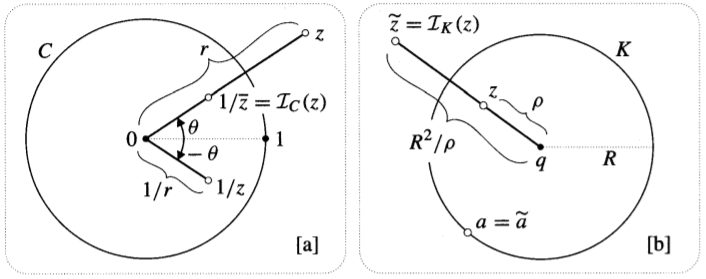
\includegraphics[scale=0.7]{fig_1}
        \label{f1}
    \end{figure}

    \item Line $L$ divides plane into two parts, $\mc{R}_L$ (reflection in $L$) interchanges those parts, $\mc{R}_L(L) = L$, $\mc{R}_L(\mc{R}_L(z)) = z$; $\mc{I}_K$ shares all three properties. As $K$ gets larger or the point to be inverted/reflected comes closer to $K$, $\mc{I}_K$ behaves as $\mc{R}_K$.

    \begin{figure}[h!]
        \centering
        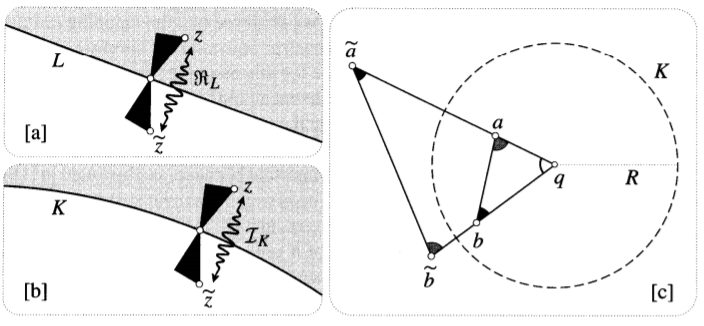
\includegraphics[scale=0.7]{fig_2}
        \label{f2}
    \end{figure}

    \item $\td{a} = \mc{I}_K(a)$, $\td{b} = \mc{I}_K(b)$, $[q\td{a}][qa] = R^2 = [qb][q\td{b}]$, $aqb \sim \td{b}q\td{a}$, $[\td{a}\td{b}]/[ab] = [q\td{a}]/[qb]$, $[\td{a}\td{b}] = ([ab]R^2)/([qa][qb])$.

    \item $L$ pass through $q$ then $\mc{I}_K(L)=L$; $L$ does not pass through $q$ then $\mc{I}_K(L) = K'$ where $K'$ is a circle through $q$, tangent to which at $q$ is parallel to $L$. $K_1$,$K_2$ with centre $q$ then $[q\td{z}_2]/[q\td{z}_1] = R_1^2/R_2^2 = k$, so, $\mc{I}_{K_2} = \mc{D}_{q}^{k} \circ \mc{I}_{K_1}$.

    \begin{figure}[h!]
        \centering
        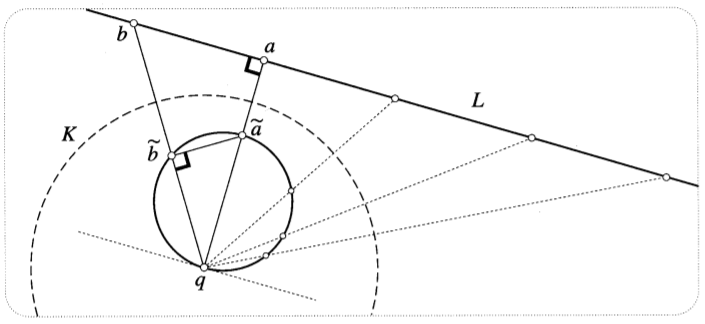
\includegraphics[scale=0.7]{fig_3}
        \label{f3}
    \end{figure}

    \item $K'$ passing through $q$ then $\mc{I}_K(K') = L$ where $L$ is parallel to tangent to $K'$ at $q$; $K'$ doesn't pass through $q$ then $\mc{I}_K(K') = K''$ where $K''$ doesn't pass through $q$.

    \begin{figure}[h!]
        \centering
        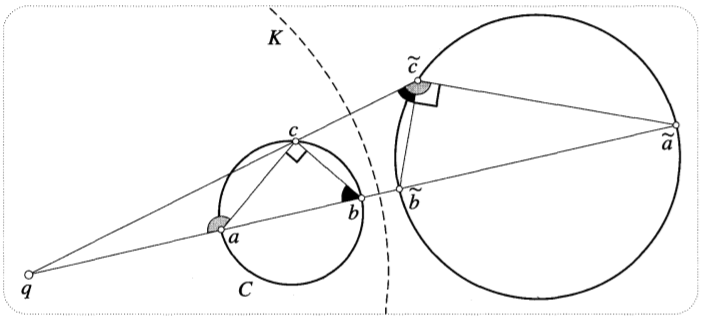
\includegraphics[scale=0.7]{fig_4}
        \label{f4}
    \end{figure}

    \item $K' \perp K$ then $\mc{I}_K(K') = K'$. $K'\perp K, K'' \perp K$ s.t. $K'$ and $K''$ intersect at $z_1, z_2$, then $I_{K}(z_1) = z_2$; $\td{z} = I_{K}(z)$ is the second intersection point of any two circles passing through $z$ and $\perp$ to $K$.
    \item As $R \rto \infty$, $I_{K}(z) = (iR\bar{z})/(\bar{z}+iR) = \bar{z}/(1-(i\bar{z}/R)) \rto \bar{z} = \mc{R}_L(z)$; As $z$ gets closer to a point $p$ (say $0$) on circle ($R$ is fixed) and $|z|<R$, $\mc{I}_K(z) = \bar{z} + i\bar{z}^2/R + \ldots \rto \bar{z}$.

    \begin{figure}[h!]
        \centering
        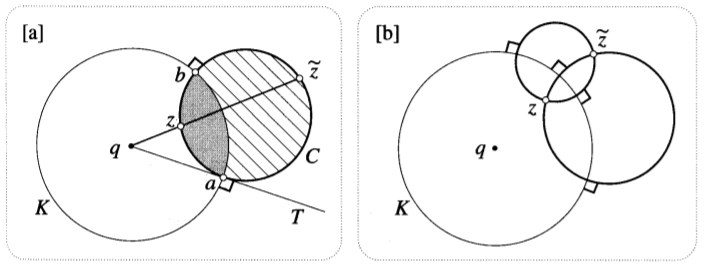
\includegraphics[scale=0.7]{fig_5}
        \label{f9}
    \end{figure}

    \item Conformal at $p$: When transformation preserves sign and magnitude of the angle between any two curves sufficiently smooth at $p$; Anticonformal at $p$: Magnitude preserved, sign reversed; Conformal map: Conformal for all $p$; Anticonformal map: Anti conformal for all $p$; Isogonal map: Magnitude preserved for all $p$, can't say anything about sign.

    \begin{figure}[h!]
        \centering
        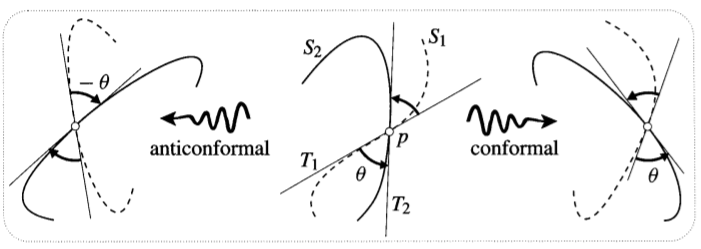
\includegraphics[scale=0.7]{fig_6}
        \label{f6}
    \end{figure}

    \item Geometric inversion is anticonformal (draw $\perp$ circle to $K$ passing through $z$ at a specific angle). Complex inversion is conformal. Even number of reflections (in lines or circles) is conformal, odd is anticonformal.

    \begin{figure}[h!]
        \centering
        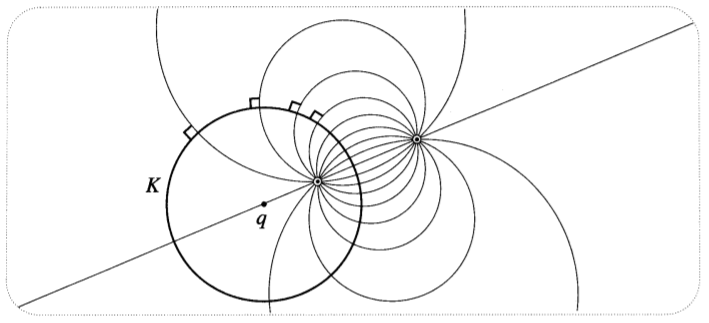
\includegraphics[scale=0.7]{fig_7}
        \label{f7}
    \end{figure}

    \begin{figure}[h!]
        \centering
        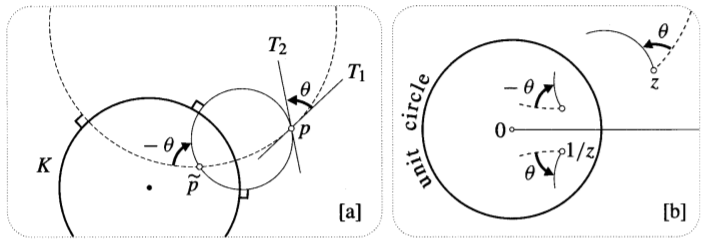
\includegraphics[scale=0.7]{fig_8}
        \label{f8}
    \end{figure}

    \item Inversion maps any pair of $\perp$ circles to another pair of $\perp$ circles; If $a$ and $b$ are symmetric wrt $K$ then $\td{a},\td{b},\td{K}=\mc{I}_J(a,b,K)$, $\td{a}$ and $\td{b}$ are symmetric wrt $\td{K}$.

    \begin{figure}[h!]
        \centering
        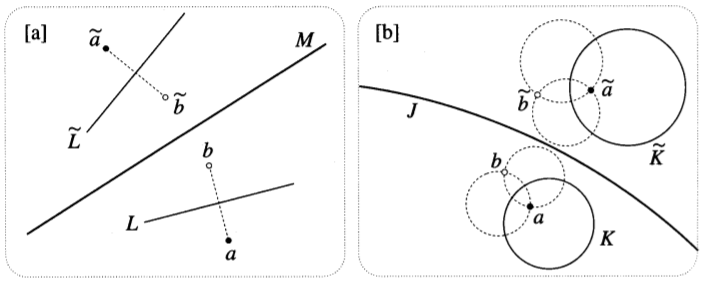
\includegraphics[scale=0.7]{fig_9}
        \label{f9}
    \end{figure}

    \item Analogous results for inversion in a sphere; Let $S_1$ and $S_2$ be intersecting spheres, and let $C_1$ and $C_2$ be the great circles in which these spheres intersect a plane $\prod$ passing through their centres. Then $S_1 \perp S_2 \iff C_1 \perp C_2$.

    \begin{figure}[h!]
        \centering
        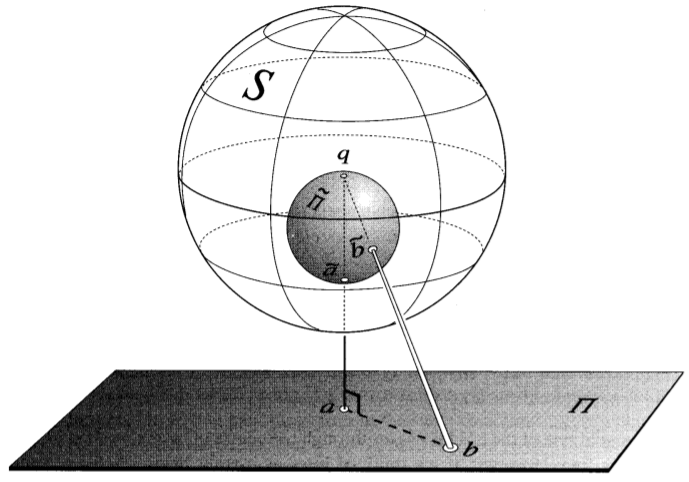
\includegraphics[scale=0.7]{fig_10}
        \label{f10}
    \end{figure}

    \begin{figure}[h!]
        \centering
        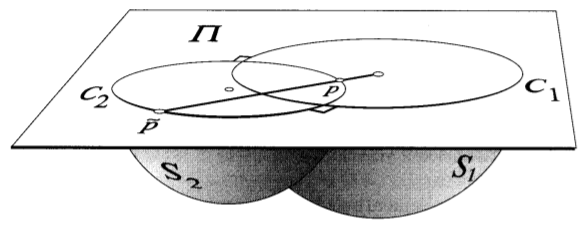
\includegraphics[scale=0.7]{fig_11}
        \label{f11}
    \end{figure}

    \item Plotemy's theorem $[ab][cd] + [ad][bc] = [ac][bd]$ where $a,b,c,d$ lie on a circle.

    \begin{figure}[h!]
        \centering
        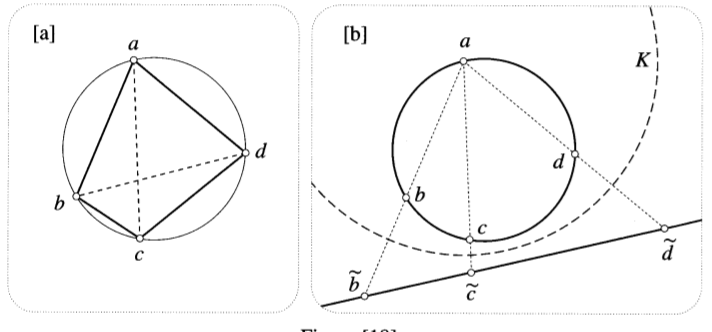
\includegraphics[scale=0.7]{fig_12}
        \label{f12}
    \end{figure}

    \item Extended complex plane = complex plan with a point $\infty$; Stereographic projection: Angle preserving (conformal (if sense of angle on $\Sigma$ by observer inside it)) mapping from extended complex plane to unit sphere $\Sigma$. Stereographic image of a line in the plane is a circle on $\Sigma$ passing through $N = \infty$. Circles on plane are mapped to circles on $\Sigma$.
    
    \begin{figure}[h!]
        \centering
        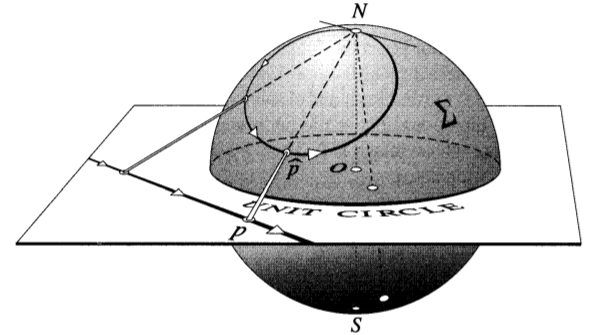
\includegraphics[scale=0.7]{fig_13}
        \label{f13}
    \end{figure}

    \begin{figure}[h!]
        \centering
        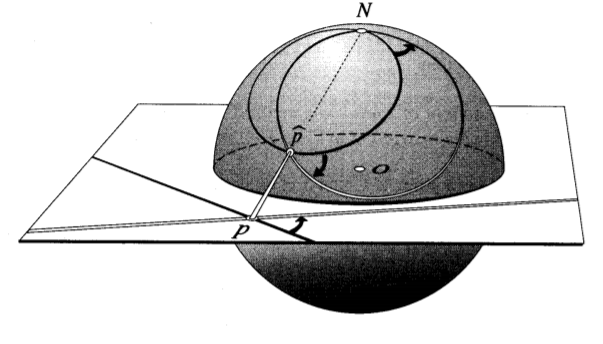
\includegraphics[scale=0.7]{fig_14}
        \label{f14}
    \end{figure}

    \item If $K$ is sphere of radius $\sqrt{2}$ centred at $N$ then stereographic projection of plane is nothing but its inversion in $K$; This is another reason why steregraphic projection preserves circles.

    \begin{figure}[h!]
        \centering
        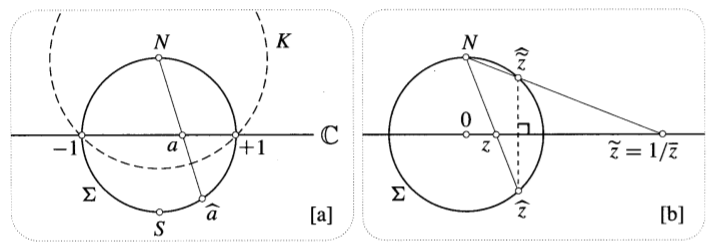
\includegraphics[scale=0.7]{fig_15}
        \label{f15}
    \end{figure}

    \item Transformation on stereographic image of complex plane corresponding to: complex conjugation is reflection of $\Sigma$ in vertical plane through real axis; geometric inversion is reflection of $\Sigma$ in its equitorial plane; complex inversion is rotation of $\Sigma$ with $\pi$ about real axis.

    \item Transferring a function from complex plane to $\Sigma$ can tell about its behaviour at $\infty \equiv N$; Complex inversion is conformal everywhere; $z\rto z^2$ is conformal everywhere except at $0$ and $N = \infty$; Such points where conformality of an otherwise conformal map breaks down are called critical points; To investigate conformality of $f(z)$ at $\infty$, take $F(z) = f(1/z)$ and check its conformality at $O$.

    \item Stereographic formulae: Given Cartesian coordinates of $z$ as $x+iy$, and Cartesian coordinates of its stereographic image on $\Sigma$ as $(X,Y,Z)$, we have, $x+iy = (X+iY)/(1-Z)$ and $X+iY = 2z/(1+|z|^2)$ where $Z = (|z|^2-1)/(|z|^2+1)$; Also, if polar coordinates of stereographic image are $(\phi,\theta)$ where $\theta$ measures angle around $Z$-axis and $\phi$ is the angle subtended at the centre of $\Sigma$ by points $N$ and $\hat{z}$, then, $z = e^{i\theta}\cot(\phi/2)$; $\hat{p}$ and $\hat{q}$ are antipodal on $\Sigma$ then $q = -1/\bar{p}$.

    \begin{figure}[h!]
        \centering
        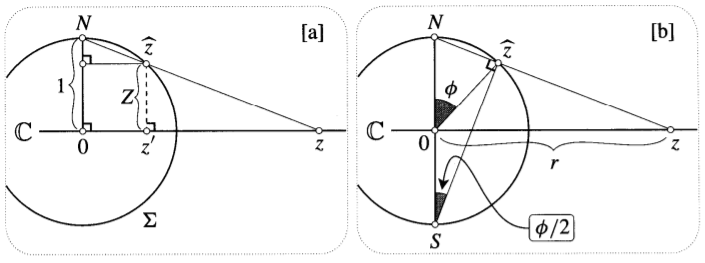
\includegraphics[scale=0.7]{fig_16}
        \label{f16}
    \end{figure}

    \item M.T. map circles to circles, are conformal, if two points are symmetric wrt a circle then their images are symmetric wrt image circle, maps an oriented circle $C$ to an oriented circle $\td{C}$ s.t. region to the left of $C$ is mapped to the region to the left of $\td{C}$.

    \begin{figure}[h!]
        \centering
        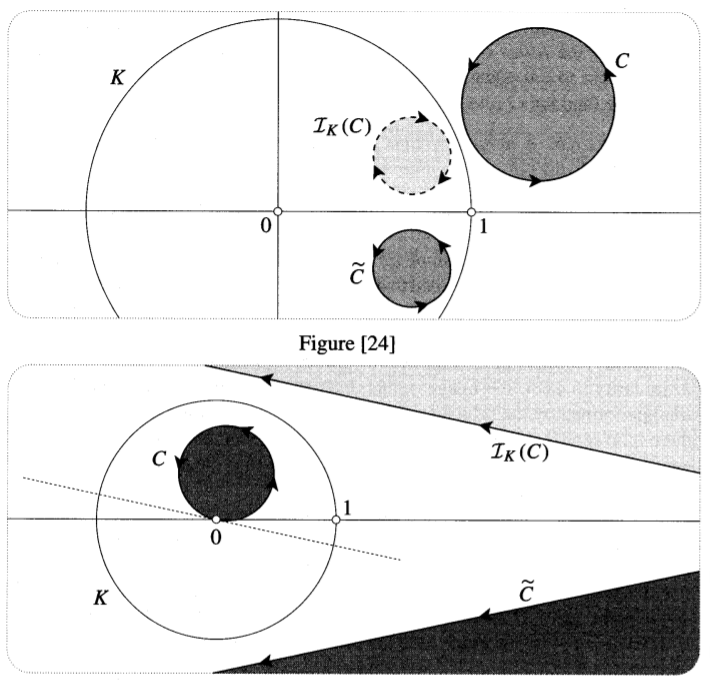
\includegraphics[scale=0.7]{fig_17}
        \label{f17}
    \end{figure}

    \item There exist a unique M.T. sending any three points to any other three points; $ad-bc=1$ then M.T. is normalized; set of M.T. forms a group under composition; $z=M(z)$ is a quadratic in $z$, so, with exception of identity mapping, a $M.T.$ has atmost two fixed points, this fact is used to prove uniqueness part; if $c \neq 0$ then both fixed points lie on a finite plane; if $c = 0$ then $M(z) = Az+B$, which is a similarity, has a fixed points at $\infty$;
    
    \item Transfer $M(z) = e^{i\theta}z$ on $\Sigma$ to see that origin centered circles are invariant curves, origin originating rays map to another such ray, and fixed points are $0$ and $\infty$: Such M.T. is called elliptic M.T.; transfer $M(z) = \rho z$ on $\Sigma$ to see that origin centered circles map to another such circle, origin originating rays are invariant curves, and fixed points are $0$ and $\infty$: Such M.T. is called hyperbolic M.T.; Transfer $M(z) = \rho e^{i\theta}z$ to see the combined effect, $0$ and $\infty$ are fixed points: Such M.T. is called loxodromic M.T.; $M(z) = z+b$ has lines parallel to $b$ as invariant curves and only $\infty$ as its fixed point: Such M.T. is called parabolic M.T.; A M.T. has a fixed point at $\infty$ $\iff$ it is a similarity $M(z) = az+b$; $\infty$ is the sole fixed point $\iff$ it is a translation $M(z) = z+b$.
    
    \begin{figure}[h!]
        \centering
        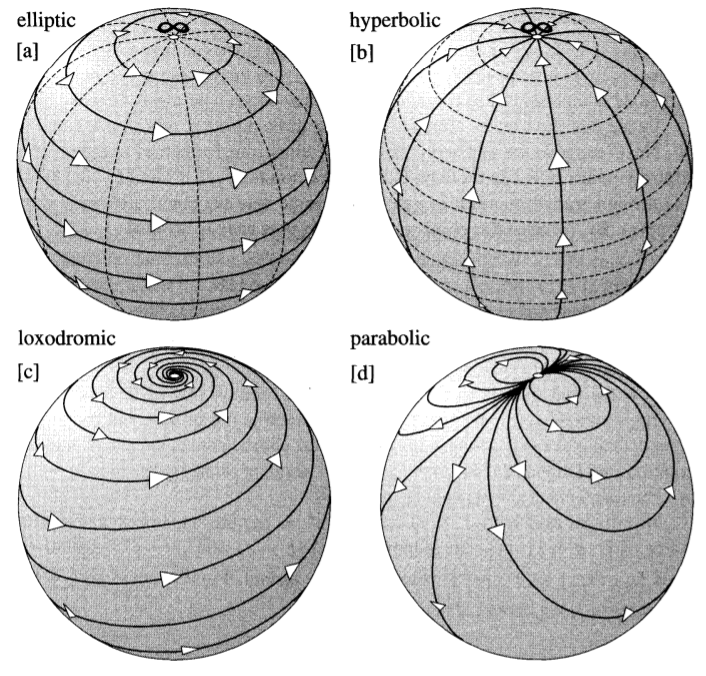
\includegraphics[scale=0.7]{fig_18}
        \label{f18}
    \end{figure}
    
    \item M.T. taking $q,r,s$ to $q',r',s'$ is given by $M'(z) = M^{-1}_{q',r',s'} \circ M_{q,r,s} (z)$ where $M_{q,r,s} = [z,q,r,s] = ((z-q)(r-s))/((z-s)(r-q))$ is a M.T. mapping $q\rto 0$, $r \rto 1$, $s \rto \infty$; $[z,q,r,s]$ is called cross-ratio; A point $p$ lies on the circle through $q,r,s$ $\iff$ $Im[p,q,r,s] = 0$; if $q,r,s$ induce positive orientation to circle then $z$ lies outside $\iff Im[p,q,r,s] < 0$ and inside if $Im[p,q,r,s] > 0$.

    \begin{figure}[h!]
        \centering
        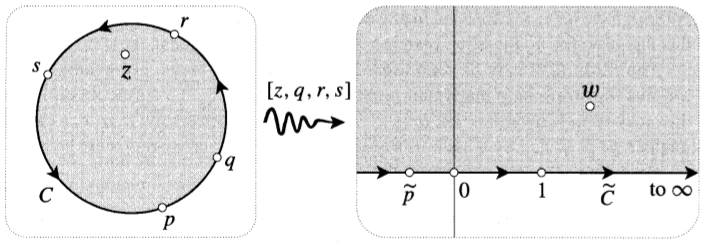
\includegraphics[scale=0.7]{fig_19}
        \label{f19}
    \end{figure}

    \item M.T. in matrix form $[a,b; c,d]$ which is non-unique; if M.T. is normalized then matrix form is unique upto sign; check following in matrix form: Identity M.T., normalization coefficient as determinant, normalized $\times$ normalized $=$ normalized, composition of M.T., inverse of M.T.; M.T. are linear transformations, only they act on homogeneous coordinates in $\C^2$; $z = \zeta_1/\zeta_2$ is a fixed point of $M(z)$ $\iff$ $[\zeta_1,\zeta_2]^T$ is evec of $[M]$; Check with matrix form that if $\infty$ is a fixed point then $c = 0$; Suppose $M(z)$ is normalized then $det([M]) = 1$, so, $det([M]-\lambda I) = \lambda^2-(a+d)\lambda+1=0$; $\lambda_1\lambda_2=1$ and $\lambda_1+\lambda_2=a+d$.
    
    \item Two vectors in $\C^2$ are $\perp$ $\iff$ they are homogeneous coordinates of antipodal points on $\Sigma$; A linear transformation $[R]$ analogous to a rotation must preserve inner product: $<[R]p,[R]q> = <p, q>$, so, $[R]^{*}[R] = I$; We get form of $[R] = [a, b; -\bar{b}, \bar{a}]$ and therefore the most general rotation of $\Sigma$ can be expressed as $R(z) = (az+b)/(-\bar{b}z+\bar{a})$.
    
    \item M.T. $M(z)$ with two fixed points $\xi_{+}$ and $\xi_i$; Consider family of circles through them as $C_1$ and family of circles s.t. each circle is $\perp$ all circles of $C_1$ as $C_2$; Note that $\xi_+$ and $\xi_i$ are symmetric wrt to a circle in $C_2$; $F(z) = (z-\xi_+)/(z-\xi_{-})$ sends $\xi_+ \rto 0$ and $\xi_{-}\rto \infty$; $C_1$ circles become straight lines from origin and $C_2$ circles become concentric origin centred circles; $w = M(z)$ in $z$-plane and in $w$-plane $\td{w}=\td{M}(\td{z})$ so that $\td{M}(\td{z}) = F(M(F^{-1}(\td{z})))$; Two fixed points, so, $\td{M}(z) = m z$ where $m = \rho w^{i\alpha}$; $m$ is the multiplier of $M(z)$; $M(z)$ is elliptic if $m = e^{i\alpha}$ - $C_1$ circles permutate among themselves and $C_2$ circles are invariant, $\alpha = (m/n)2\pi$ then period of $M$ is $n$.

    \begin{figure}[h!]
        \centering
        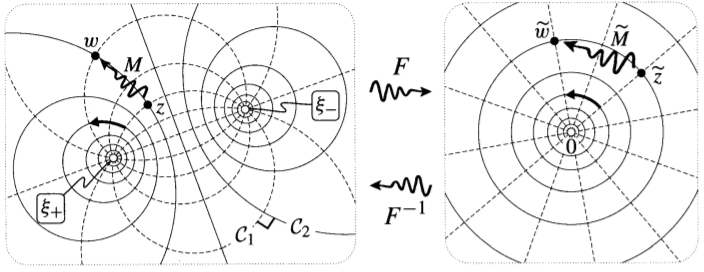
\includegraphics[scale=0.7]{fig_20}
        \label{f20}
    \end{figure}

    \begin{figure}[h!]
        \centering
        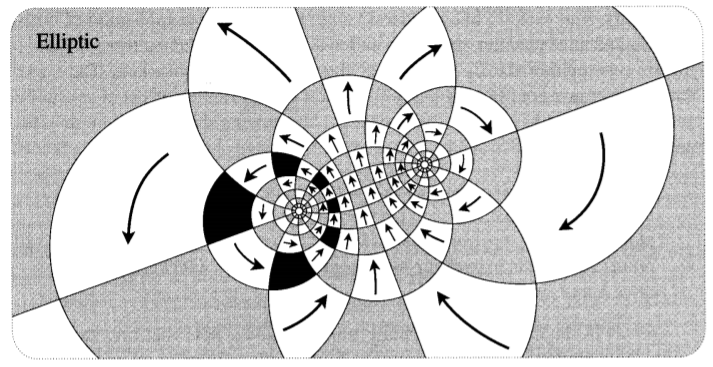
\includegraphics[scale=0.7]{fig_21}
        \label{f21}
    \end{figure}
    
    \item $M(z)$ is hyperbolic if $m = \rho$: $C_1$ circles are invariant and $C_2$ circles permutate, $\rho < 1$ is contraction and movement is from $\xi_{-}$ to $\xi_{+}$ and analogously with $\rho > 1$.
    
    \begin{figure}[h!]
        \centering
        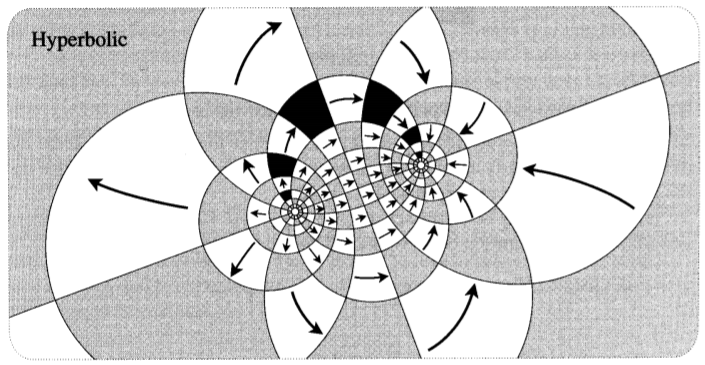
\includegraphics[scale=0.7]{fig_22}
        \label{f22}
    \end{figure}
    
    \item $M(z)$ is loxodromic if $m = \rho e^{i\alpha}$; $m$ is the multiplier associated with $\xi_+$ and $1/m$ is the multiplier associated with $\xi_{-}$; Locally, i.e. near $\xi_+$ the effect of $M(z)$ is just dilative rotation $m$ and near $\xi_{-}$ the effect of $M(z)$ is again dilative rotation $1/m$.
    
    \begin{figure}[h!]
        \centering
        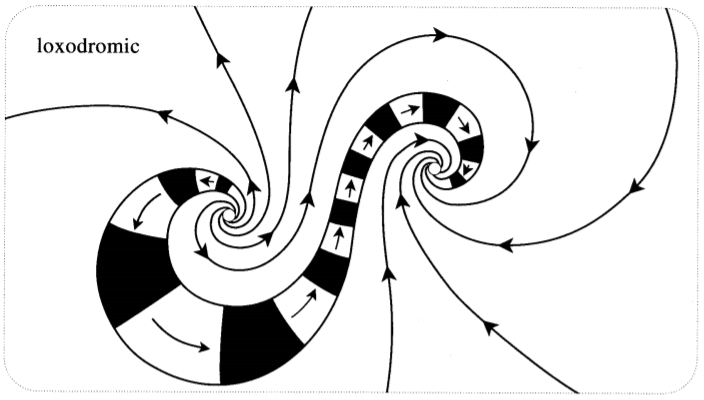
\includegraphics[scale=0.7]{fig_23}
        \label{f23}
    \end{figure}

    \item M.T. $M(z)$ with one fixed point $\xi$; $C_1$ and $C_2$ be two $\perp$ families of circle passing through $\xi$, so, $\perp$ at the second point of intersections too; $G(z)=1/(z-\xi)$ sends $\xi \rto \infty$; $C_1$ and $C_2$ are mapped to two $\perp$ families of lines; $\td{M}(\td{z}) = G(M(G^{-1}(\td{z})))$; $\infty$ is only fixed point, so, $\td{M}(\td{z}) = \td{z}+T$; $C_1$ circles permutate and $C_2$ circles permutate; $M(z)$ is said to be parabolic in such case; Also, normalized $M(z)$ is parabolic $\iff (a+d) = \pm 2$ so $\xi = (a-d)/2c$ and we get $T = \pm c$.

    \begin{figure}[h!]
        \centering
        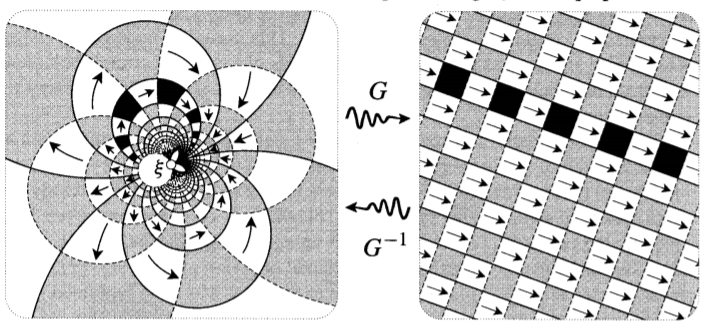
\includegraphics[scale=0.7]{fig_24}
        \label{f24}
    \end{figure}

    \item Since $M(z)$ maps $z=\infty$ to $w=a/c$ the multiplier can be computed by $(a/c-\xi_{+})/(a/c-\xi_{-})=m(z-\xi_+)/(z-\xi_-) = m$; Using $det([\td{M}]) = det([F][M][F^{-1}]) = det([M])$, $\td{M}(\td{z}) = m\td{z}$ and normalized form of $[\td{M}] = [\sqrt{m}, 0; 0, 1/\sqrt{m}]$ we get $tr([\td{M}]) = tr([F][M][F^{-1}]) = tr([M]) = a+d$, so, $\sqrt{m}+1/\sqrt{m} = a+d$; $M(z)$ is elliptic $\iff$ $a+d$ is real and $|a+d|<2$; $M(z)$ is parabolic $\iff$ $(a+d)=\pm 2$; $M(z)$ is hyperbolic $\iff$ $a=d$ is real and $|a+d|>2$; $M(z)$ is loxodromic $\iff$ $a+d$ is complex.

    \item If a fixed points of $M(z)$ is represented as an evec with eval $\lambda$ of a normalized matrix $[M]$ then the multiplier associated with the fixed point is given by $m = 1/\lambda^2$. The two reciprocal values of $m$ equal to the two reciprocal vallues of $\lambda^2$. Easy exercise to show that $m_+ = 1/\lambda_+^2$ where $\lambda_+$ is the eval corresponsing to evec/fixed point $\xi_+$.

    \item Composition of any two reflections is a M.T.; Composition of $2$ reflections is a non-loxodromic M.T. and composition of $4$ reflections is a loxodromic M.T.; Elliptic case - $m=e^{i\alpha}$ then $M(z) = \mc{I}_B(\mc{I}_A(z))$ where $A$ and $B$ are two circles from $C_1$ s.t. angle from $A$ to $B$ is $\alpha/2$.; Hyperbolic case - $m=\rho$ then $M(z)=\mc{I}_B(\mc{I}_A(z))$ where $A$ and $B$ are two circles of Appolonius with limit points $\xi_{\pm}$ s.t. $r_B/r_A = \sqrt{\rho}$ - if a point moves s.t. ratio of its distance from $\xi_+$ and $\xi_-$ is constant then the point moves on a circle, $r_A = |\td{z}| = |F(z)| = |(z-\xi_+)/(z-\xi_-)|$; Parabolic case - $M(z) = \mc{I}_B(\mc{I}_A(z))$ where $A$ and $B$ are circles that touch each other at $\xi$ s.t. the distance between parallel line $G(A)$ and $G(B)$ is $T/2$.

    \begin{figure}[h!]
        \centering
        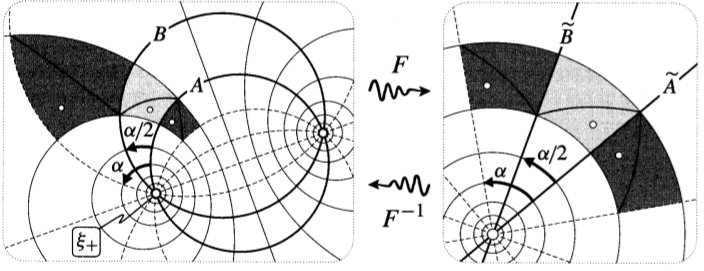
\includegraphics[scale=0.7]{fig_25}
        \label{f25}
    \end{figure}

    \begin{figure}[h!]
        \centering
        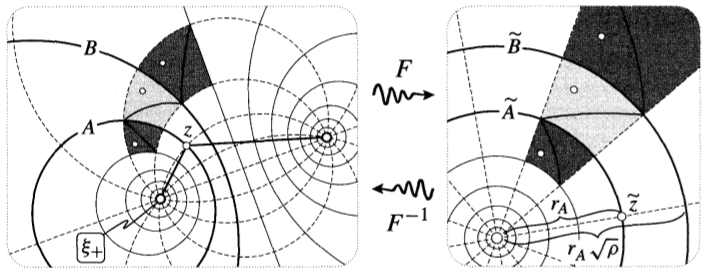
\includegraphics[scale=0.7]{fig_26}
        \label{f26}
    \end{figure}

    \begin{figure}[h!]
        \centering
        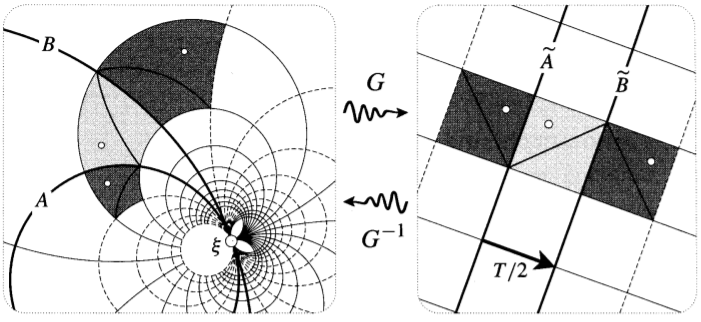
\includegraphics[scale=0.7]{fig_27}
        \label{f27}
    \end{figure}

    \item Automorphisms of unit disc. An automorphism of a region $R$ of the complex plane is a one-to-one, conformal mapping of $R$ to itself. A M.T. has six degress of freedom (need image of $3$ fixed complex numbers to specify). M.A. of unit disc $D$ have three degrees of freedom (need three angles to specify images of three fixed points on the boundary of disc). Another way to fill up 3 degrees of freedom: specify which point $a$ inside $D$ is to be mapped to origin and which point $p$ on $C$ is image of the point $1$.

    \begin{figure}[h!]
        \centering
        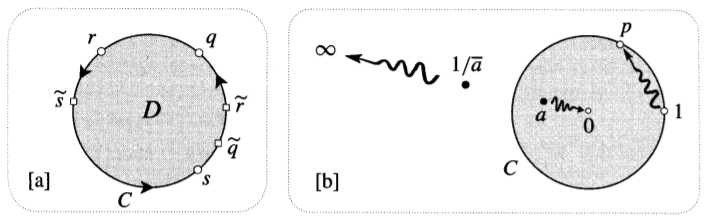
\includegraphics[scale=0.7]{fig_28}
        \label{f28}
    \end{figure}
    
    \item If two M.A. $M$ and $N$ map two interior points to the same image points, then $M=N$; Since $C$ is mapped to itself by $M$, the symmetry principle tells us that if a pair of points are symmetric wrt to $C$ then so are their images. Since $a$ is mapped to $0$, $1/\bar{a}$ will map to $\infty$. Thus, form of $M$ is $M = k(z-a)/(\bar{a}z-1)$ where $k$ is a constant. Also, $p=M(1)$. So, $1 = |p| = |k|(|1-a|)/(|\bar{a}-1|) = |k|$. So $k=e^{i\phi}$. Choice of $p$ is equivalent to choice of $\phi$. $M_{0}^{\phi}=e^{-i\phi}$ which rotates $D$ about origin by $\pi+\phi$. $M_{a}^{\phi} = R^{\phi}_{0} \circ M_{a}^{0}$. $M_{a}^{0}\equiv M_{a}$; $M_a$ swaps $0$ and $a$. This is the only M.A. with this property. $M_a = R_L \circ I_J$ where $J$ is the circle orthogonal to $C$ which swaps $a$ and $0$ and has $1/\bar{a}$ as centre, and $L$ is the line passing through $0$ and $a$ (and so through $1/\bar{a}$). Fixed points $\xi_{\pm}$ are intersection points of $J$ and $L$, and so they are symmetric with repect to $C$. Since reflections occur in orthogonal circles through these points, $M_a$ is elliptic and $m=e^{i\pi}$ associated with both $\xi_{pm}$. So, $M_a$ is involuntary and any pair of points $z$, $M_a(z)$ is swapped by $M_a$. $M_a$ can also be expressed as $I_{L'} \circ I_{J'}$ where $J'$ and $L'$ are any two circles through $\xi_+$ that are orthogonal to $C$. If $\Phi \equiv 2\cos^{-1}|a|$, then $M_a^{\phi}$ is elliptic if $|\phi|<\Phi$, parabolic if $|\phi|=\Phi$ and hyperbolic if $|\phi|>\Phi$.

    \begin{figure}[h!]
        \centering
        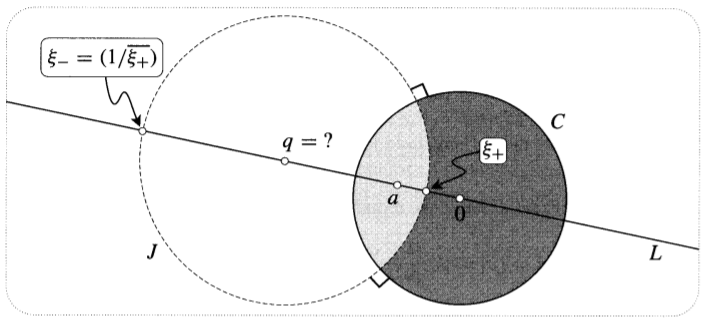
\includegraphics[scale=0.7]{fig_29}
        \label{f29}
    \end{figure}

    \begin{figure}[h!]
        \centering
        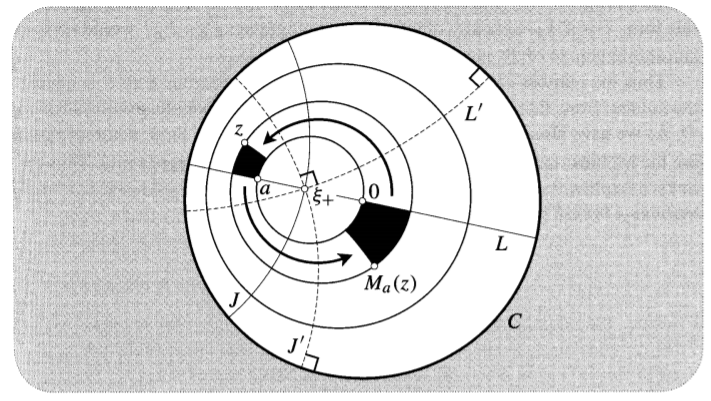
\includegraphics[scale=0.7]{fig_30}
        \label{f30}
    \end{figure}

    \item Riemann's Mapping Theorem: Any simply connected region $R$ (other than the entire plane) may be mapped one-to-one and conformally to any other such region $S$. It is sufficient to establish this in case of $S$ being $D$, for if, $F_R$ is a one-to-one conformal mapping from $R$ to $D$, and $F_S$ is a one-to-one mapping of $S$ to $D$, then $F_S^{-1} \circ F_R$ is a one-to-one conformal mapping of $R$ to $S$. $\td{F}_R \circ F_R^{-1}$ would always be some automorphism $M$ of $D$ so that $\td{F}_R = M \circ F_R$. Number of one-to-one conformal mappings from $R$ to $S$ is equal to the number from $R$ to $D$, which in turn is equal to the number of automorphisms of $D$. We will show that these automorphisms are $M_{a}^{\phi}$ which form a $3$ parameter family. This imples that there exist a $3$-parameter family of one-to-one conformal mappings from $R$ to $S$.
\end{enumerate}
\end{document}
